%!TEX program = xelatex
\documentclass[cn,hazy,pku,12pt,normal,math=newtx,cite=super]{elegantnote}
\usepackage{draftwatermark}
\SetWatermarkText{Z.C. Wang} % 设置水印文本
\SetWatermarkScale{1} % 设置水印大小
\SetWatermarkColor[gray]{0.9} % 设置水印颜色

\title{实验九\quad 偶极矩的测定\\
\Large{稀溶液法测定正丁醇的偶极矩}}

\author{王子宸\quad 210001873\\
周四19组\quad 8号}
\institute{化学与分子工程学院}

\expdate{\zhdate{2023/10/12}}
\temperature{20.9 \si{^{\circ}C}}
\pressure{101.44 \si{kPa}}

\usepackage{array,longtable,subcaption}
\usepackage[version=4]{mhchem}

\pagecolor{white}
\begin{document}

\maketitle

\keywords{国家精品课 \quad 物理化学实验 \quad 偶极矩 \quad 正丁醇 \quad 介电常数 \quad 折射率}

\abstracts{
本实验通过稀溶液法测定正丁醇的偶极矩。首先,使用数字密度仪和精密电容测量仪,测定不同浓度的正丁醇-环己烷溶液体系的密度与电容,从而求出其总摩尔极化率 $\bar{P}_2^\infty= (8.065  \pm 0.315) \times 10^{-5} \ \mathrm{~m^3\cdot mol^{-1}}$;然后使用阿贝折射仪测定正丁醇的折射率,从而求出其摩尔折射度即电子极化率为 $R=P_E=(2.2133  \pm 0.0016 )\times 10^{-5}\mathrm{~ m^3\cdot mol^{-1}}$;最终,通过计算转向极化度来计算其偶极矩,计算得到正定出浓度偶极矩为 $\mu_{\ce{\textit{n}-BuOH}}=\left (1.68 \pm 0.045 \right )\mathrm{~D} $
}

\newpage

\section{引言}

\subsection{实验目的与原理}


\begin{figure}[htbp]
    \centering
    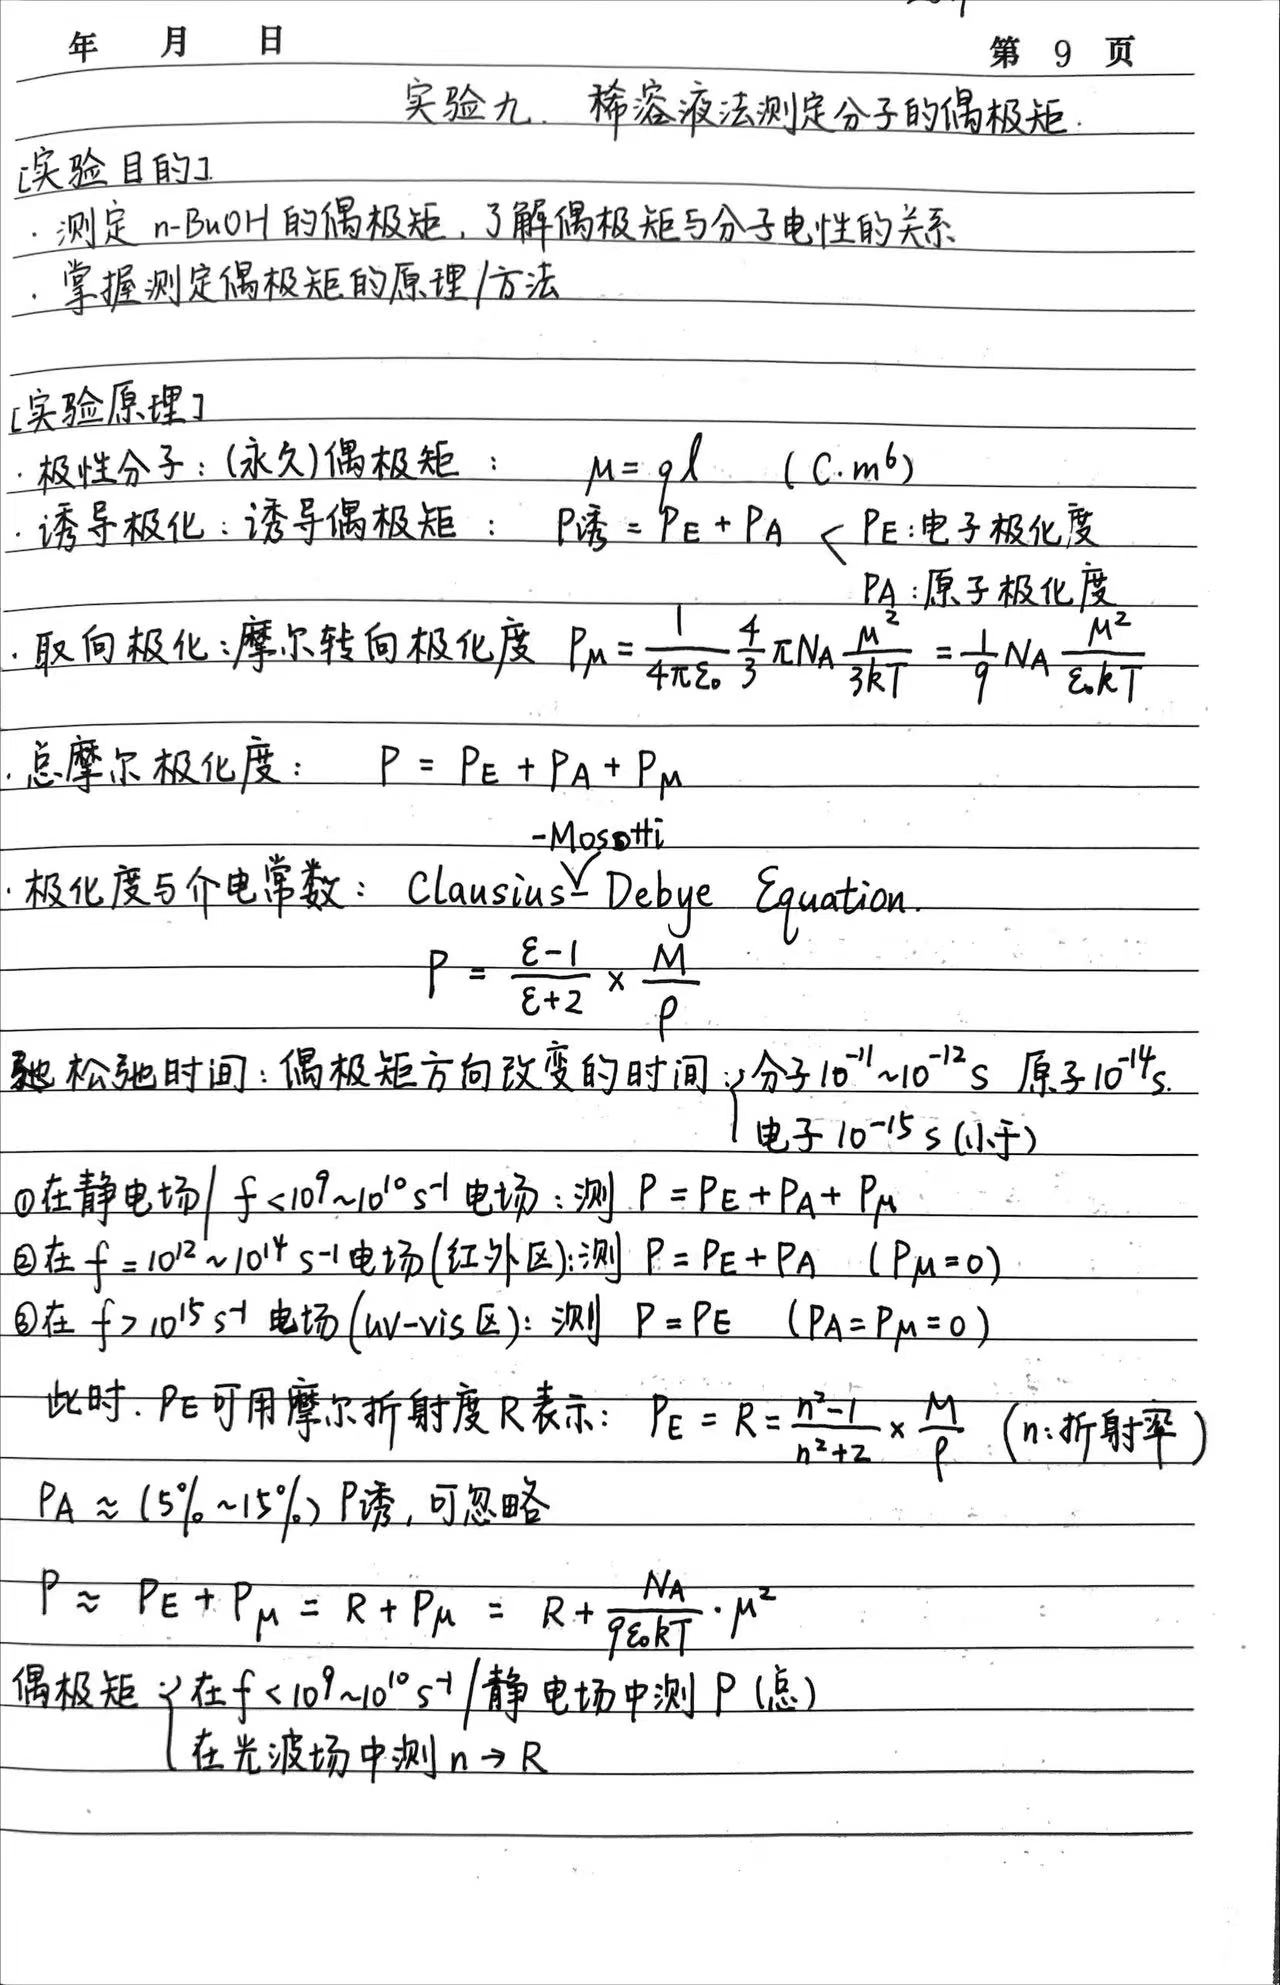
\includegraphics[width=.77\textwidth]{figures/0-1-1.jpg}
\end{figure}

\begin{figure}[htbp]
    \centering
    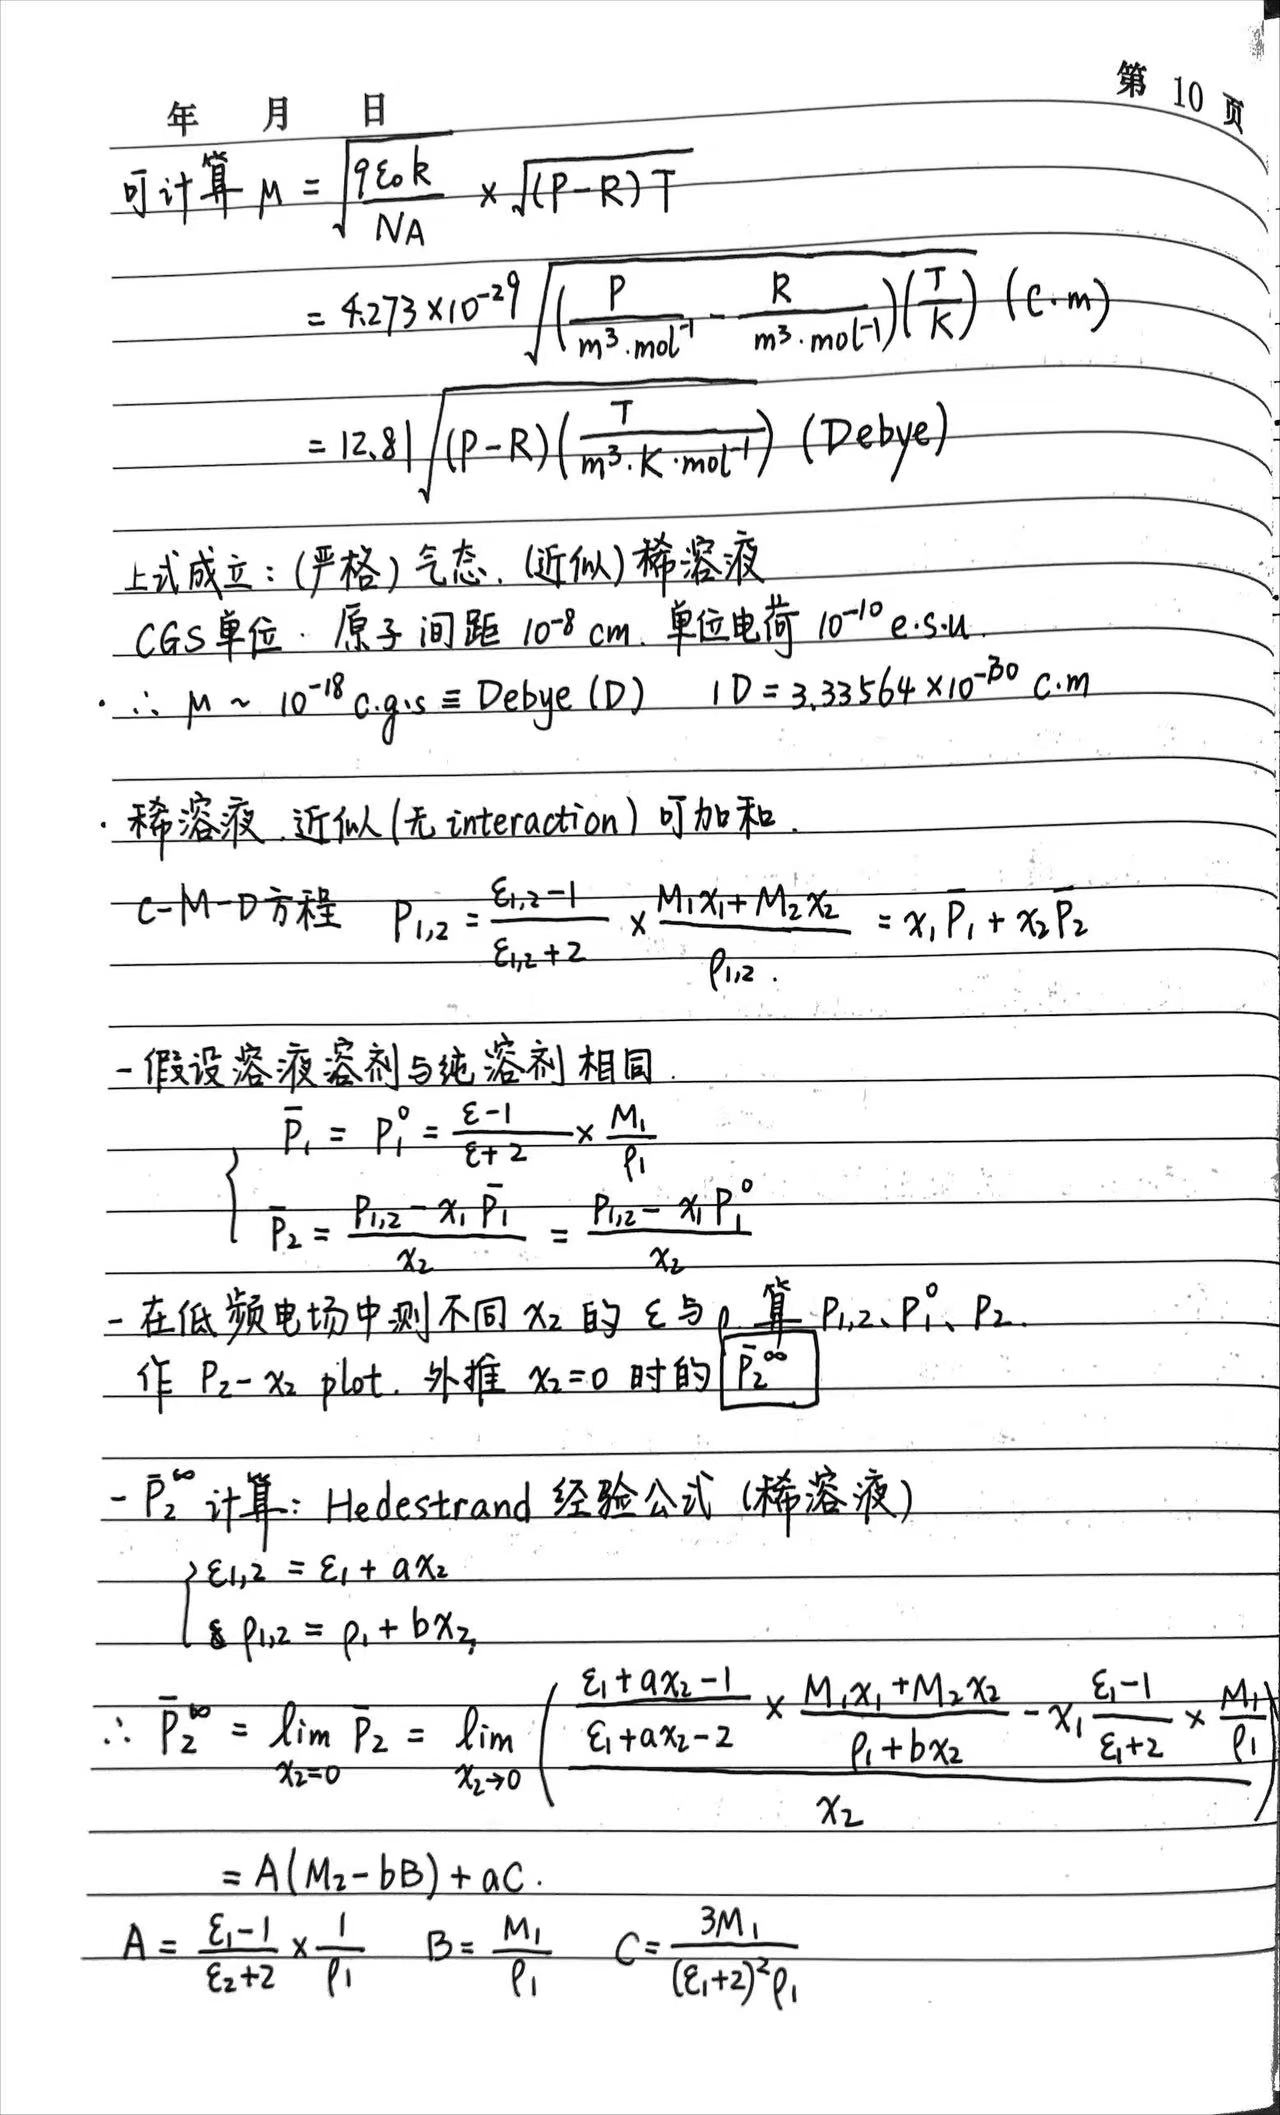
\includegraphics[width=.8\textwidth]{figures/0-1-2.jpg}
\end{figure}

\begin{figure}[htbp]
    \centering
    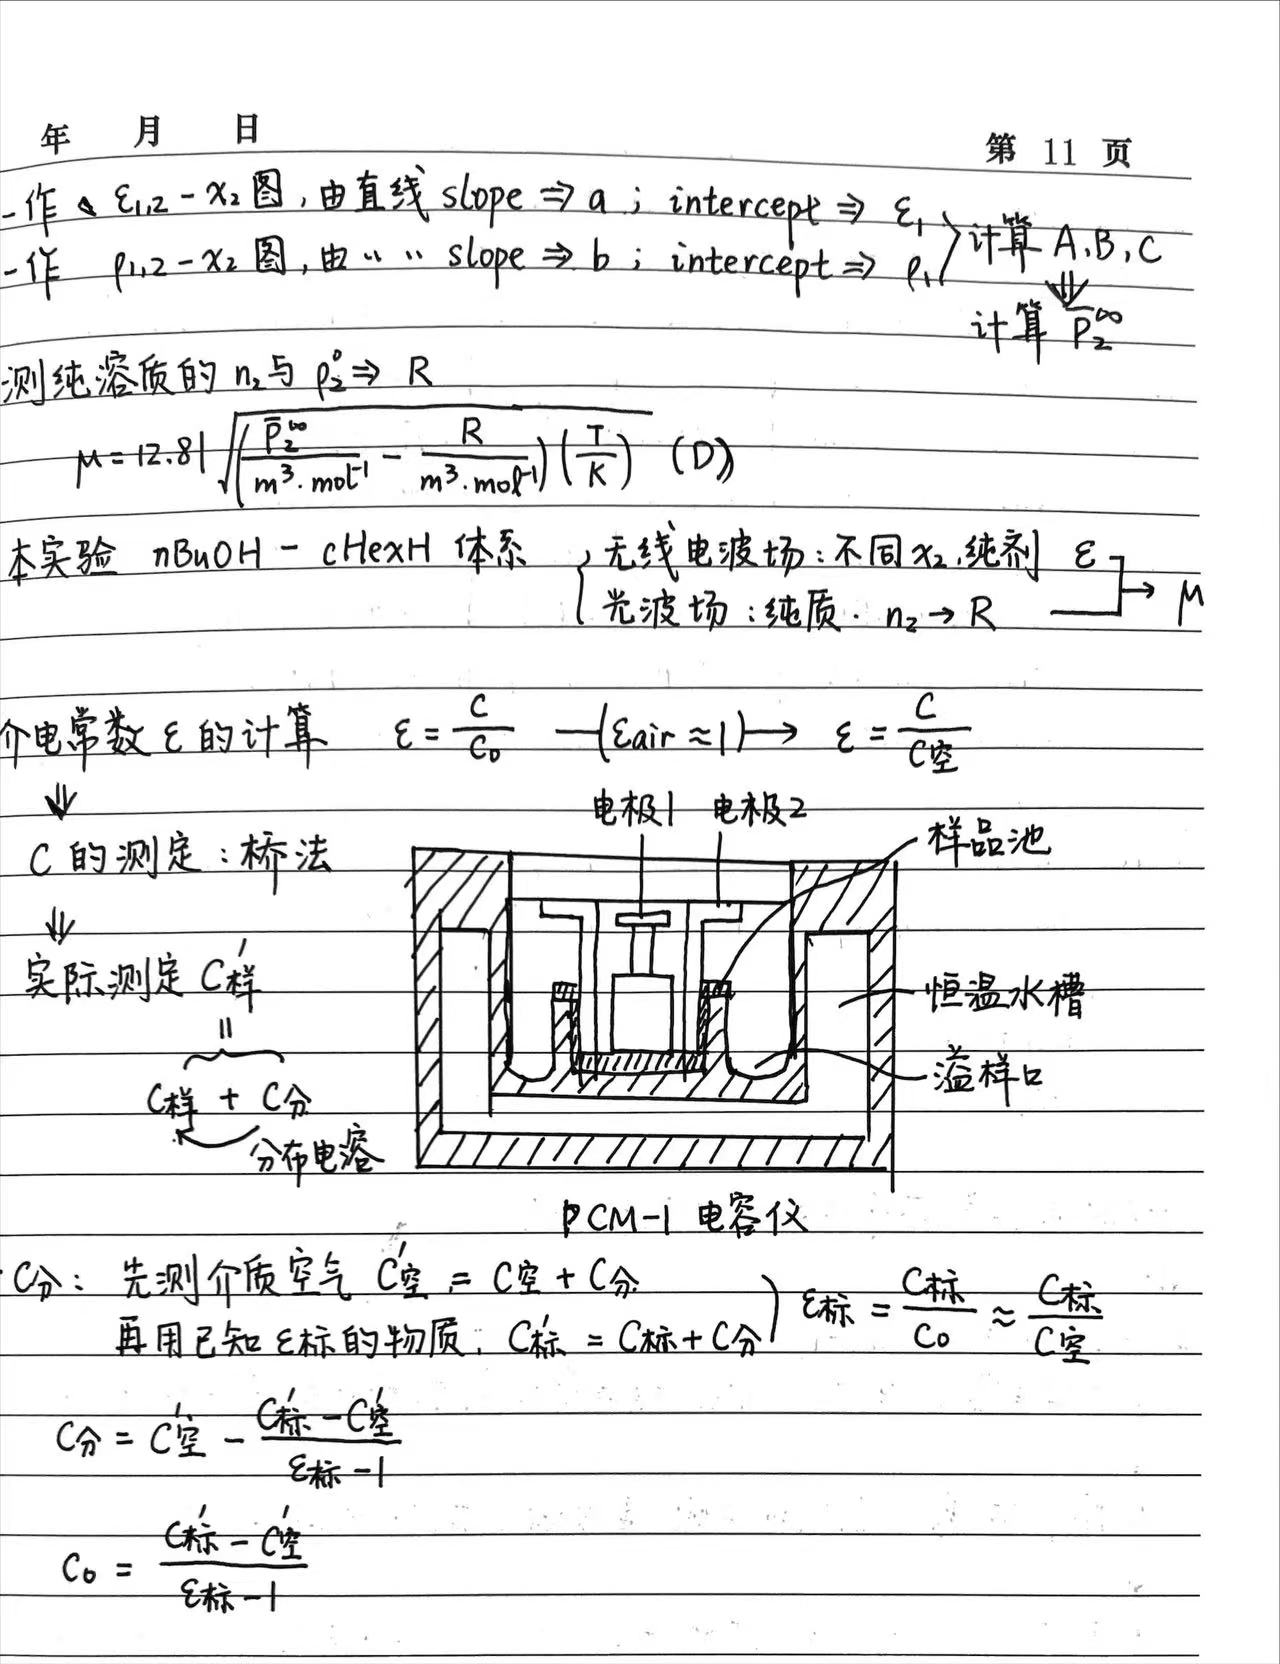
\includegraphics[width=.8\textwidth]{figures/0-1-3.jpg}
    \caption{预习报告:实验目的与原理}
\end{figure}

\newpage
\section{实验}

\subsection{主要仪器与药品}

\begin{figure}[htbp]
    \centering
    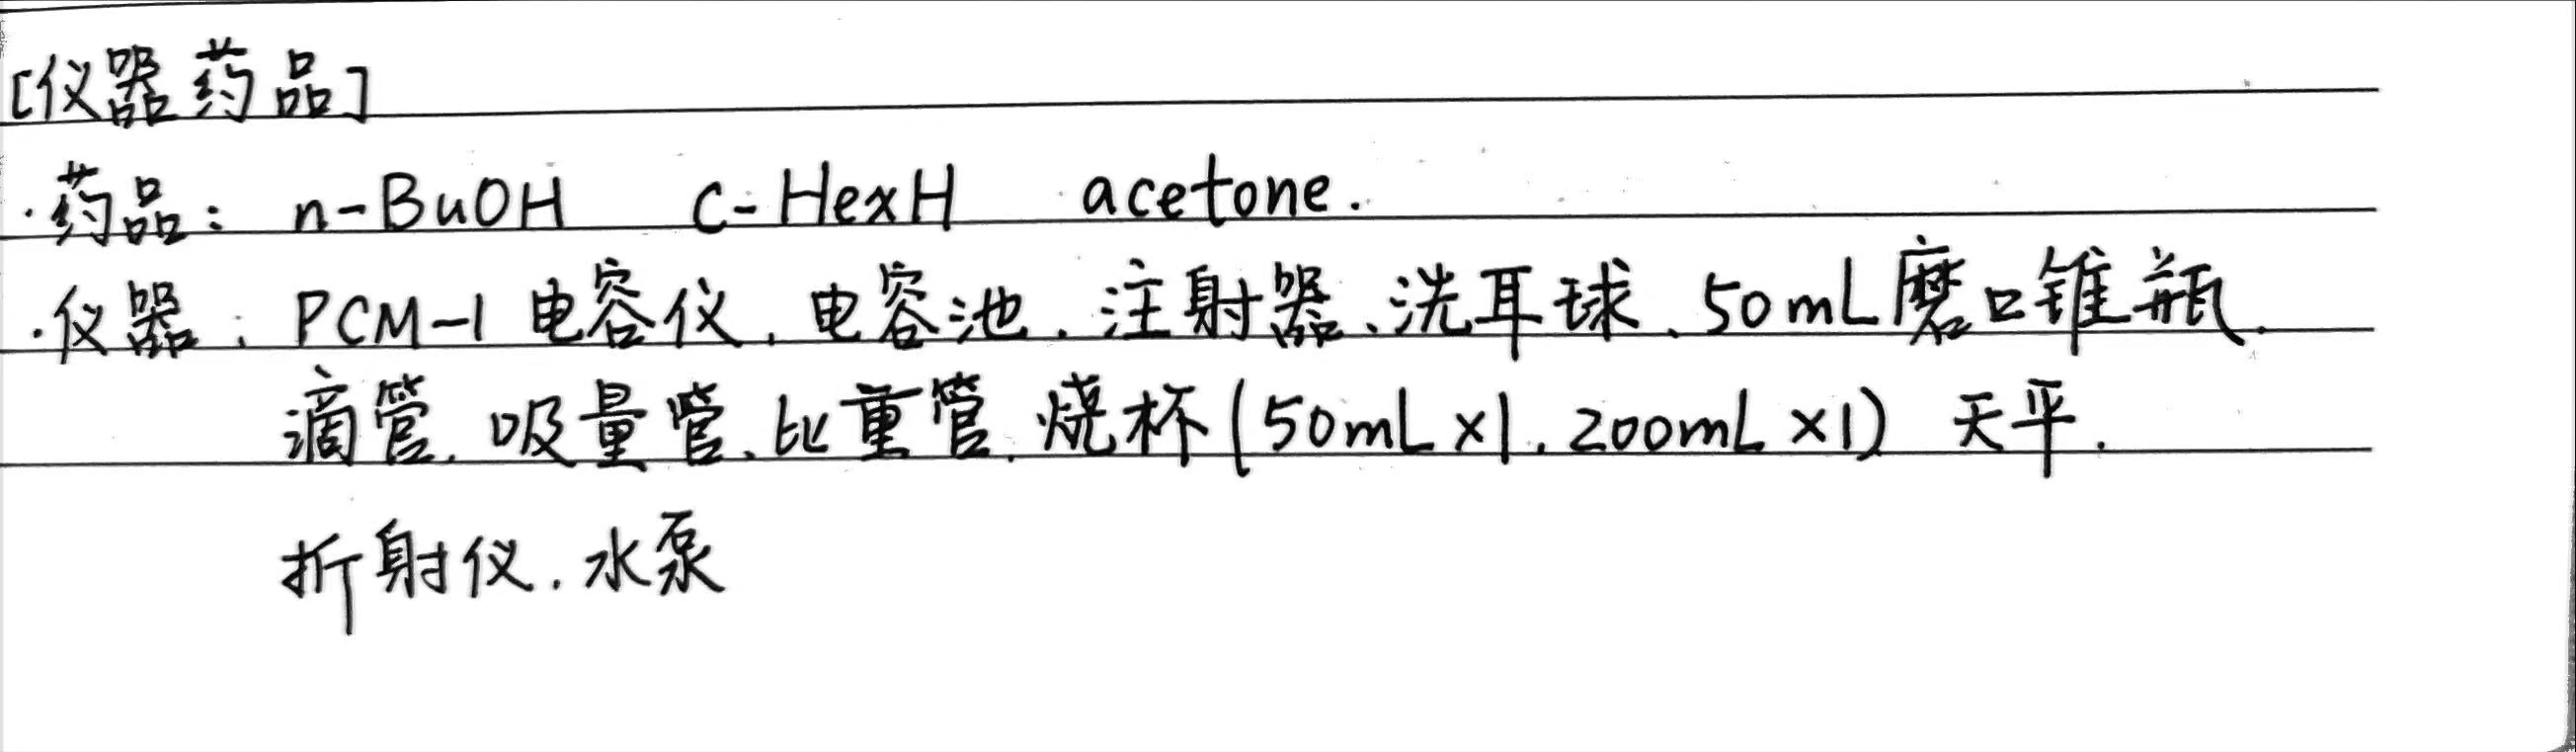
\includegraphics[width=.8\textwidth]{figures/0-2.jpg}
    \caption{预习报告:主要仪器与药品}
\end{figure}

\subsection{实验步骤与条件}

在实验开始前,需要计算出不同摩尔浓度的正丁醇(\ce{\textit{n}-BuOH})-环己烷(\ce{CyH})溶液中,需要实际加入的正丁醇、环己烷质量。

首先,假设正丁醇与环己烷混合后体积不变,假设其总量为$1\mathrm{~mol}$,根据摩尔比、相对分子量、密度,计算正丁醇体积$V_1^\prime$与环己烷体积$V_2^\prime$,进而求得正丁醇在溶液中的体积百分比$v_1$:
\begin{align*}
    V_1^\prime &= \frac{x_1 \times 1 \mathrm{~mol} \times M_{\ce{\textit{n}-BuOH}}}{\rho_{\ce{\textit{n}-BuOH}}} = 92.21x_1\mathrm{~mL}\\
    V_2^\prime &= \frac{x_1 \times 1 \mathrm{~mol} \times M_{\ce{CyH}}}{\rho_{\ce{CyH}}} = 107.9(1-x_1)\mathrm{~mL}\\
    v_1 &= \frac{V_1}{V_1+V_2}\times 100\%
\end{align*} 

求得正丁醇在溶液中的体积百分比之后,结合溶液的总体积($15\mathrm{~mL}$)、密度,求得需要添加的正丁醇与环己烷的体积$V_1,V_2$与质量$m_1, m_2$。
\begin{align*}
    V_1 &= V_0 \times v_1 = 15v_1\mathrm{~mL}\\
    V_2 &= V_0 \times v_2 = 15v_2\mathrm{~mL}\\
    m_1 &= \frac{V_1}{\rho_{\ce{\textit{n}-BuOH}}} = \frac{V_1/\mathrm{mL}}{0.8148} \mathrm{~mL}\\
    m_2 &= \frac{V_2}{\rho_{\ce{CyH}}} = \frac{V_2/\mathrm{mL}}{0.78} \mathrm{~mL}
\end{align*}

最终计算结果如表 \ref{fig:1}
\begin{figure}[htbp]
    \centering
    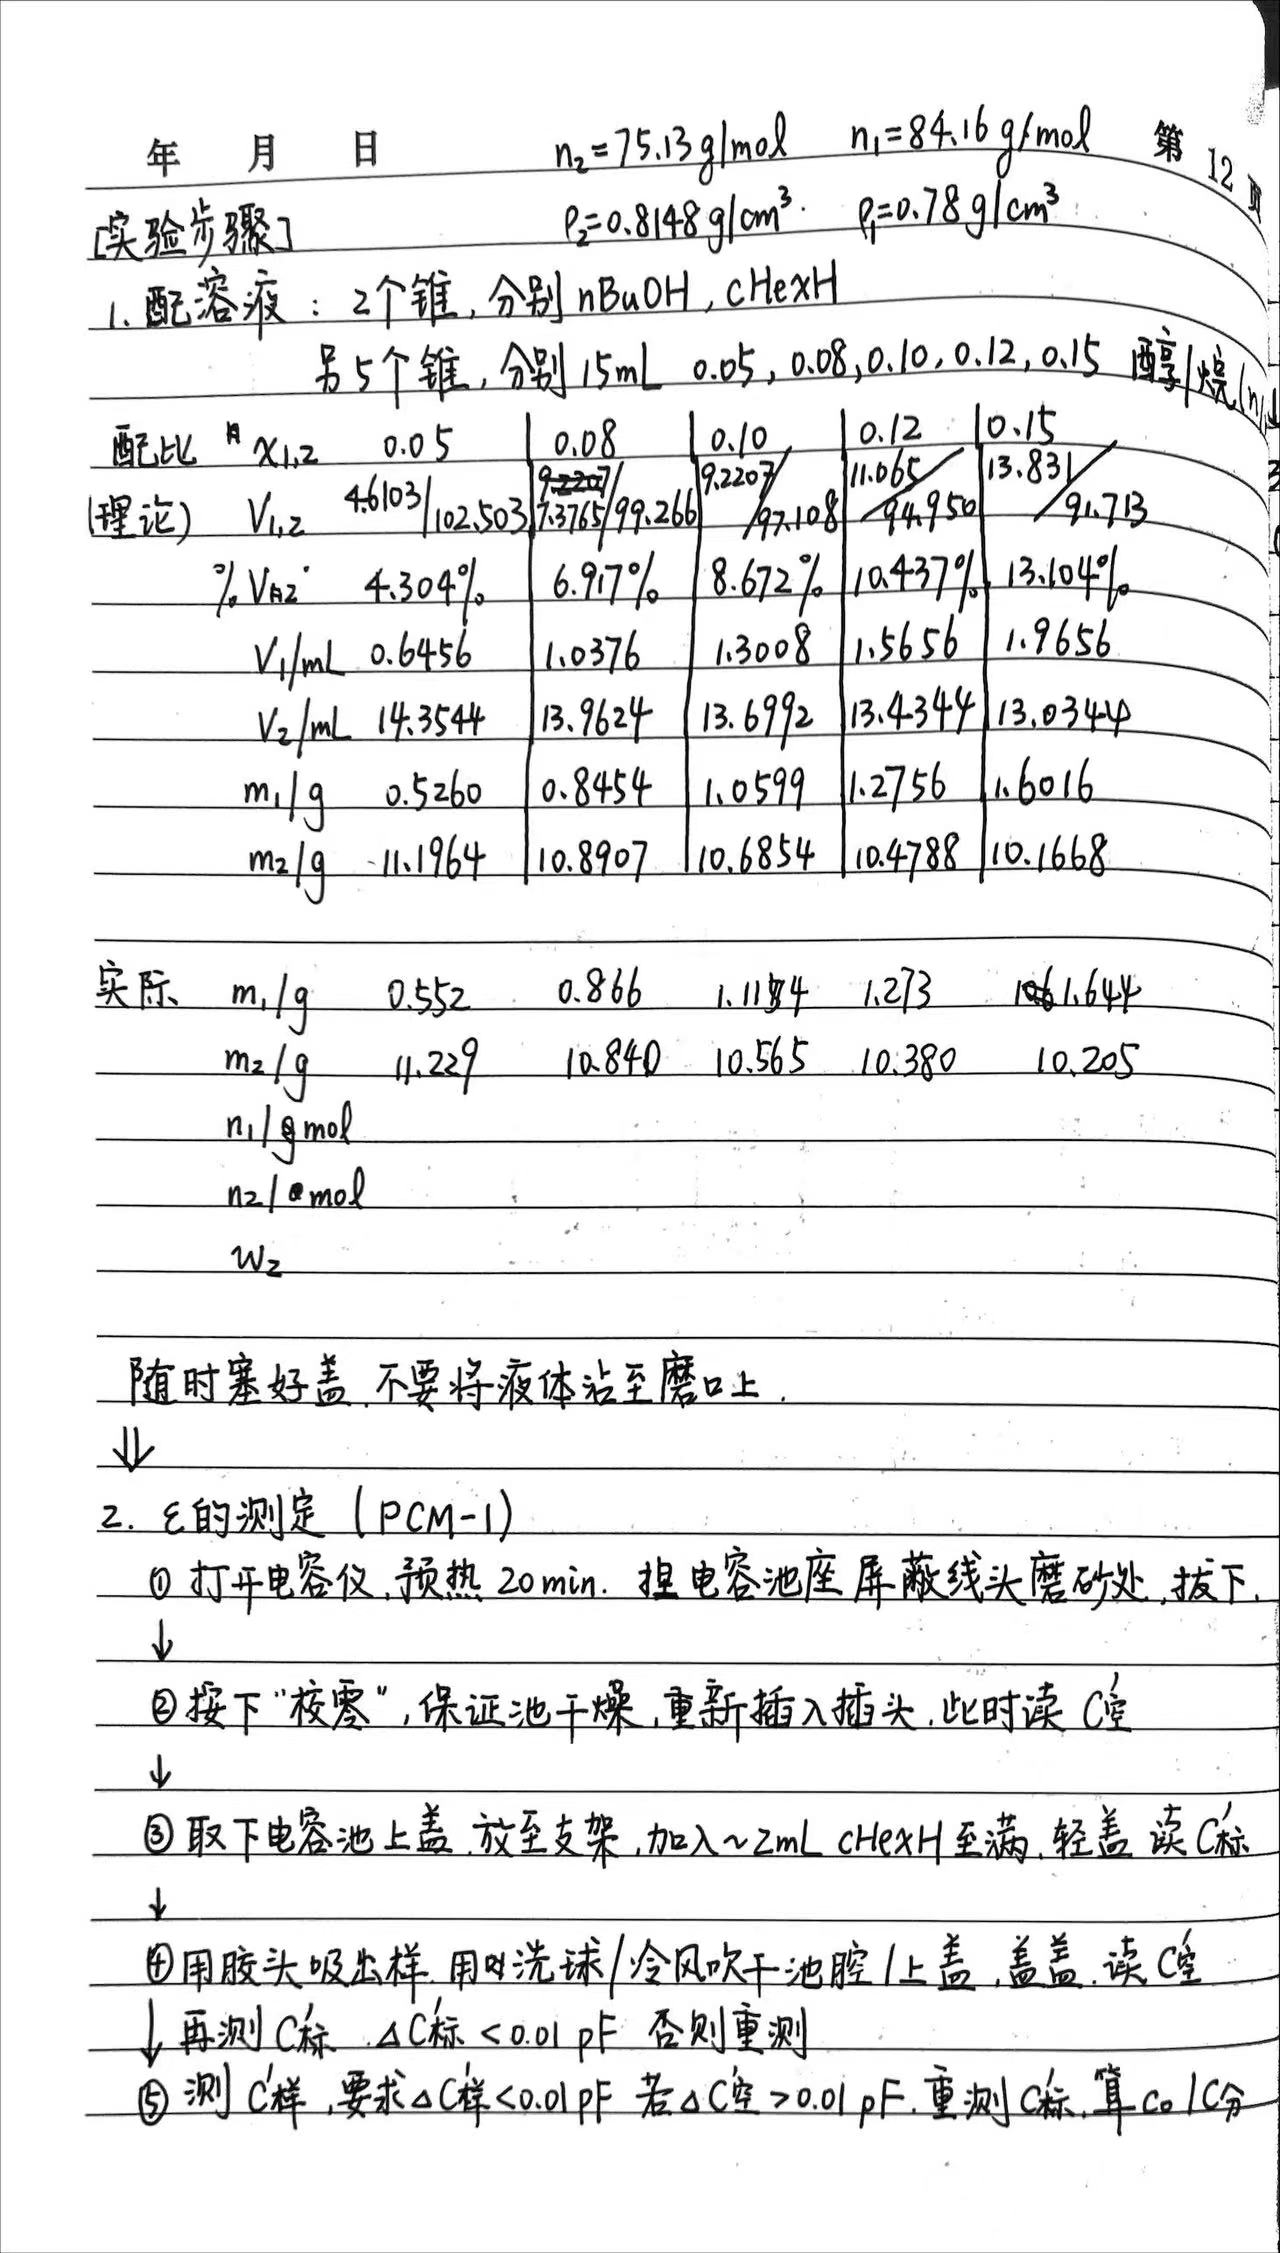
\includegraphics[width=.8\textwidth]{figures/0-3-1.jpg}
\end{figure}

\begin{figure}[htbp]
    \centering
    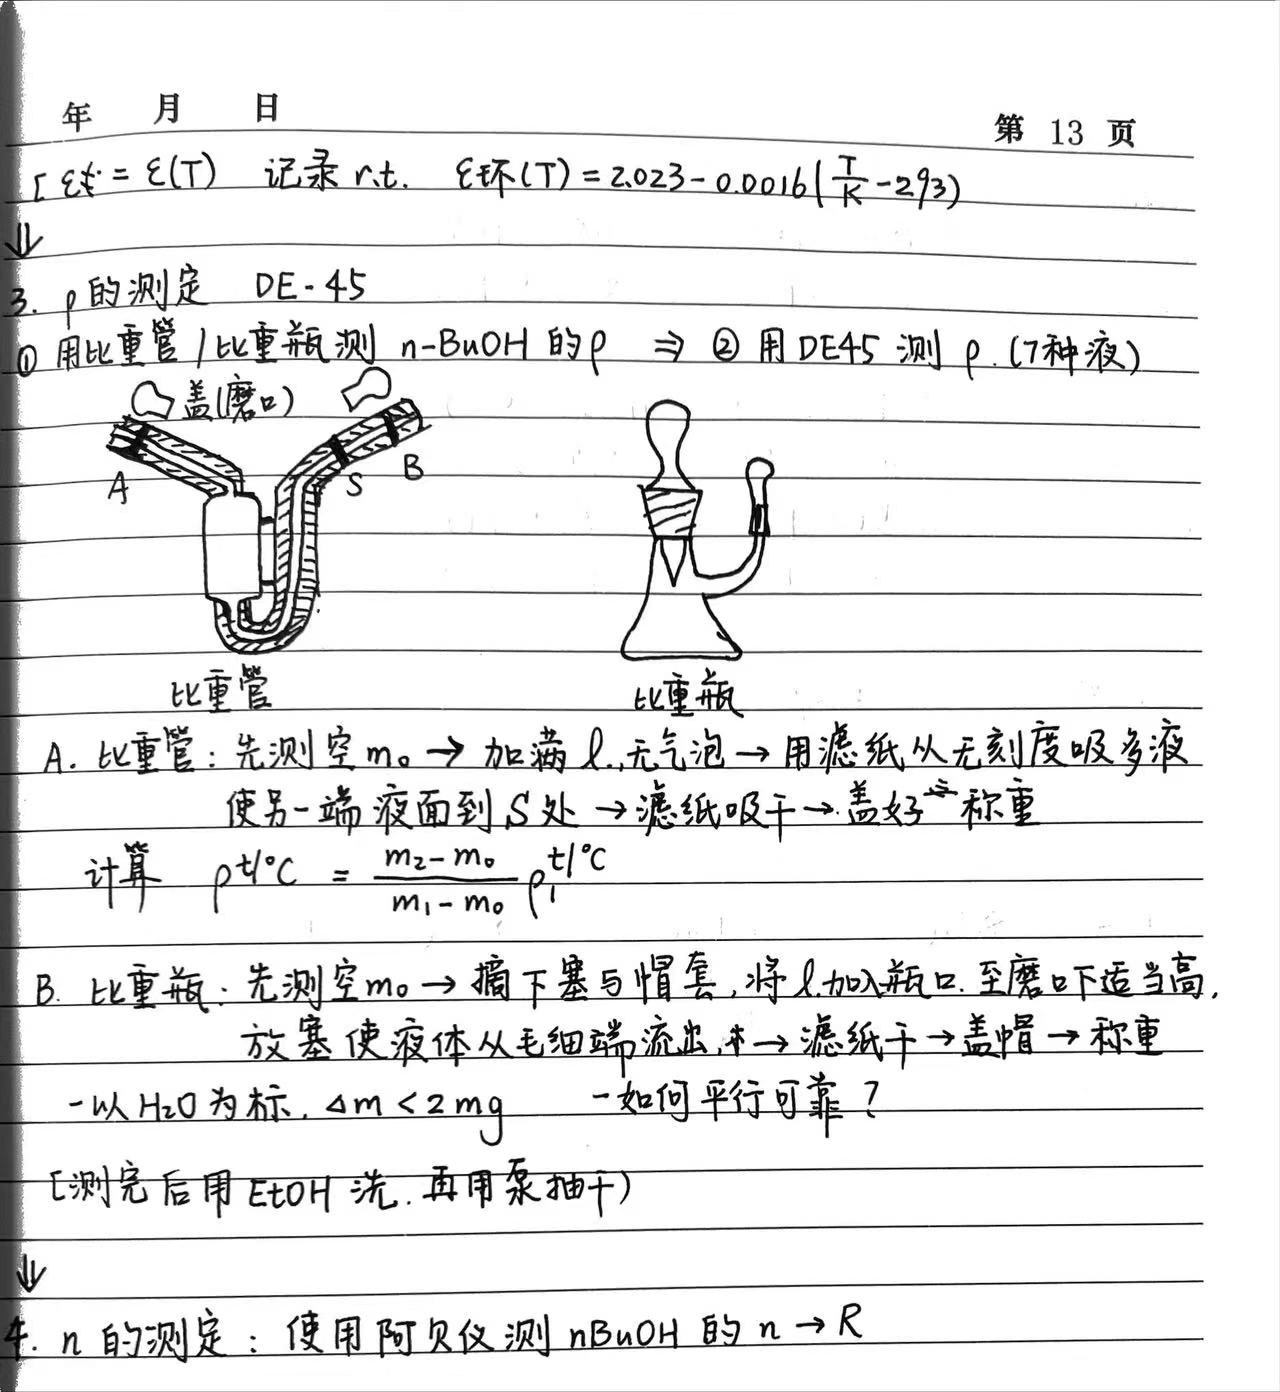
\includegraphics[width=.8\textwidth]{figures/0-3-2.jpg}
    \caption{预习报告:实验步骤与条件}
    \label{fig:1}
\end{figure}

\section{数据处理与结果呈现}

\subsection{溶液的摩尔浓度}


实际配制溶液的测量数据如表 \ref{tab:1} 所示,其中,正丁醇的摩尔分数由公式 \eqref{eq:1} 求出。
\begin{equation}\label{eq:1}
    x = \frac{\dfrac{m_{\ce{\textit{n}-BuOH}}}{74.12\mathrm{~g}}}{\dfrac{m_{\ce{\textit{n}-BuOH}}}{74.12\mathrm{~g}}+\dfrac{m_{\ce{CyH}}}{84.16\mathrm{~g}}}
\end{equation}
假设千分之一天平单次称量的允差为$0.001\mathrm{~g}$,则其误差为(为了方便书写,本实验报告中所有误差均略去单位,其单位与对应的物理量保持一致):
\begin{align*}
    \sigma_m = \frac{0.001}{\sqrt{3}} = 5.8\times 10^{-4} \\
    \sigma_{\Delta m} = \sqrt{2}\sigma_m = 8.2\times 10^{-4} 
\end{align*}
以第一组数据为例,计算溶液摩尔浓度的误差:
\begin{equation*}
x=\frac{0.01349 m_{\ce{\textit{n}-BuOH}}}{0.01349 m_{\ce{\textit{n}-BuOH}} + 0.01188 m_{\ce{CyH}}}=\frac{0.01349 \times \left(0.552\right)}{0.01349 \times \left(0.552\right) + 0.01188 \times \left(11.229\right)}=0.0529\  
\end{equation*}
\begin{equation*}
\begin{aligned}
\frac{\partial x }{\partial m_{\ce{\textit{n}-BuOH}} }&=- \frac{1.0 m_{\ce{\textit{n}-BuOH}}}{\left(m_{\ce{\textit{n}-BuOH}} + 0.8807 m_{\ce{CyH}}\right)^{2}} + \frac{0.01349}{0.01349 m_{\ce{\textit{n}-BuOH}} + 0.01188 m_{\ce{CyH}}}\\
{}&=- \frac{1.0 \times \left(0.552\right)}{\left(\left(0.552\right) + 0.8807 \times \left(11.229\right)\right)^{2}} + \frac{0.01349}{0.01349 \times \left(0.552\right) + 0.01188 \times \left(11.229\right)}=0.091\\
\frac{\partial x }{\partial m_{\ce{CyH}} }&=- \frac{0.8807 m_{\ce{\textit{n}-BuOH}}}{\left(m_{\ce{\textit{n}-BuOH}} + 0.8807 m_{\ce{CyH}}\right)^{2}}=- \frac{0.8807 \times \left(0.552\right)}{\left(\left(0.552\right) + 0.8807 \times \left(11.229\right)\right)^{2}}=-0.0045\\
\end{aligned}
\end{equation*}
\begin{equation*}
\begin{aligned}
\sigma_{x}&=\sqrt{\left(\frac{\partial x }{\partial m_{\ce{\textit{n}-BuOH}} } \sigma_{m_{\ce{\textit{n}-BuOH}}}\right)^2+\left(\frac{\partial x }{\partial m_{\ce{CyH}} } \sigma_{m_{\ce{CyH}}}\right)^2}\\
&=\sqrt{\left(0.091 \times 0.00082\right)^2+\left(-0.0045 \times 0.00082\right)^2}\\
&=\sqrt{\left(7.4 \times 10^{-5}\right)^2+\left(-3.7 \times 10^{-6}\right)^2}\\
&=7 \times 10^{-5}\
\end{aligned}
\end{equation*}
\begin{equation*}
x=\left (0.0529 \pm 7 \times 10^{-5} \right )\
\end{equation*}
最终,计算得到所有摩尔浓度的不确定度,如表 \ref{tab:1} 中所示。
\begin{table}[htbp]
    \centering
    \caption{称量数据与各溶液的实际摩尔分数}
    \begin{tabular}{cccc}
        \toprule
        $x_0$ & $m_{\ce{\textit{n}-BuOH}}/\mathrm{g}$ & $m_{\ce{CyH}}/\mathrm{g}$ & $x$\\
        \midrule
        0.05 & 0.552 & 11.229 & $0.0529 \pm 0.00007$ \\
        0.08 & 0.866 & 10.840 & $0.0832 \pm 0.00007$ \\
        0.10 & 1.114 & 10.565 & $0.107 \pm 0.00007$ \\
        0.12 & 1.273 & 10.380 & $0.122 \pm 0.00007$ \\
        0.15 & 1.644 & 10.205 & $0.155 \pm 0.00007$ \\
        \bottomrule
    \end{tabular}
    \label{tab:1}
\end{table}

%由表 \ref{tab:1},不难发现摩尔浓度的不确定度较小,在之后的计算中可以忽略。

\subsection{溶液的介电常数}\label{cap:1}

根据经验公式,环己烷的介电常数可以根据温度求出:
\begin{equation}\label{eq:8}
    \begin{aligned}
    \varepsilon_{\ce{CyH}} &= 2.023 - 0.0016\left(\frac{T}{\mathrm{K}}-293\right)\\
    &= 2.203 - 0.0016\left((273.15+20.9)-293\right)\\
    &= 2.021
\end{aligned}
\end{equation}
其中,考虑温度计的允差为 $0.1\mathrm{{}^\circ C}$,则温度计的误差为:
\begin{equation*}
    \sigma_T = \frac{0.1}{\sqrt{3}} = 0.058
\end{equation*}
但是,由于温度之前有系数0.0016,故温度测定误差对于$\varepsilon_{\ce{CyH}}$的影响可忽略不计。

测得的电容数据如表 \ref{tab:2} 所示。

假设电容计的允差为$0.01\mathrm{~pF}$,则电容计误差为:
\begin{equation*}
    \sigma_{C} = \frac{0.01}{\sqrt{3}} = 0.0057
\end{equation*}
其中,首先通过平均,得到介质为空气时电容器的电容$C_{\text{air}}^\prime$:
\begin{equation*}
    C_{\text{air}}^\prime = \bar{C}_{\text{air}}= 4.25 \mathrm{~pF}
\end{equation*}
此处对12组数据取平均,故误差为:
\begin{equation*}
    \sigma_{C_{\text{air}}} = \frac{\sqrt{12}}{12}\sigma_{C} = 0.0016
\end{equation*}
所以:
\begin{equation*}
    C_{\text{air}}^\prime = (4.25\pm 0.0016) \mathrm{~pF}
\end{equation*}

然后,根据介质为空气、环己烷时的电容,与环己烷的介电常数,计算得到电容器的分布电容$C_{\text{d}}$:
\begin{equation}\label{eq:9}
    C_{\text{d}} = C_{\text{air}}^\prime - \frac{C_{\ce{CyH}}^\prime-C_{\text{air}}^\prime}{\varepsilon_{\ce{CyH}}-1} = 4.25 -\frac{7.02-4.25}{2.021-1} = 1.537\mathrm{~pF} 
\end{equation}
分布电容的误差为:
\begin{equation*}
\begin{aligned}
\frac{\partial C_{\text{d}} }{\partial C_{\text{air}} }&=\frac{2.021}{2.021-1}=1.979=2.0\\
\frac{\partial C_{\text{d}} }{\partial C_{\ce{CyH}}^\prime }&=\frac{1}{2.021-1}=-0.979=-0.98\\
\end{aligned}
\end{equation*}
\begin{equation}\label{eq:10}
\begin{aligned}
\sigma_{C_{\text{d}}}&=\sqrt{\left(\frac{\partial C_{\text{d}} }{\partial C_{\text{air}} } \sigma_{C_{\text{air}}}\right)^2+\left(\frac{\partial C_{\text{d}} }{\partial C_{\ce{CyH}}^\prime } \sigma_{C_{\ce{CyH}}^\prime}\right)^2}\\
&=\sqrt{\left(2.0 \times 0.0016\right)^2+\left(-0.98 \times 0.0058\right)^2}\\
&=\sqrt{\left(0.0032\right)^2+\left(-0.0057\right)^2}\\       
&=0.006\  
\end{aligned}
\end{equation}
所以,分布电容为:
\begin{equation*}
C_{\text{d}}=\left (1.54 \pm 0.006 \right )\ \mathrm{~pF} 
\end{equation*}


根据电容器的分布电容$C_{\text{d}}$,计算表 \ref{tab:2} 中不同摩尔浓度正丁醇-环己烷溶液的介电常数$\varepsilon$,计算公式如式 \eqref{eq:2} ,结果如表 \ref{tab:2}。
\begin{equation}\label{eq:2}
    \varepsilon_i = \frac{C_i}{C_{\text{air}}} = \frac{\bar{C}_{1,i}-C_{\text{d}}}{\bar{C}_{\text{air}}-C_{\text{d}}} = \frac{\bar{C}_{1,i}-1.54}{\bar{C}_{\text{air}}-1.54}
\end{equation}

考虑两次测量电容均值的误差:
\begin{equation*}
    \sigma_{\bar{C}} = \frac{\sqrt{2}}{2}\sigma_C = 0.004
\end{equation*}
以第一组数据为例,计算介电常数及其不确定度:
\begin{equation*}
\varepsilon=\frac{- C_{\text{d}} + \bar{C}_{\ce{CyH}}^\prime}{- C_{\text{d}} + \bar{C}_{\text{air}}}=\frac{- \left(1.54\right) + \left(7.02\right)}{- \left(1.54\right) + \left(4.25\right)}=2.02\
\end{equation*}
\begin{equation*}
\begin{aligned}
\frac{\partial \varepsilon }{\partial \bar{C}_{\text{air}} }&=\frac{C_{\text{d}} - \bar{C}_{\ce{CyH}}^\prime}{\left(C_{\text{d}} - \bar{C}_{\text{air}}\right)^{2}}=\frac{\left(1.54\right) - \left(7.02\right)}{\left(\left(1.54\right) - \left(4.25\right)\right)^{2}}=-0.75\\
\frac{\partial \varepsilon }{\partial \bar{C}_{\ce{CyH}}^\prime }&=- \frac{1}{C_{\text{d}} - \bar{C}_{\text{air}}}=- \frac{1}{\left(1.54\right) - \left(4.25\right)}=0.37\\
\frac{\partial \varepsilon }{\partial C_{\text{d}} }&=\frac{\bar{C}_{\ce{CyH}}^\prime - \bar{C}_{\text{air}}}{\left(C_{\text{d}} - \bar{C}_{\text{air}}\right)^{2}}=\frac{\left(7.02\right) - \left(4.25\right)}{\left(\left(1.54\right) - \left(4.25\right)\right)^{2}}=0.38\\
\end{aligned}
\end{equation*}
\begin{equation*}
\begin{aligned}
\sigma_{\varepsilon}&=\sqrt{\left(\frac{\partial \varepsilon }{\partial \bar{C}_{\text{air}} } \sigma_{\bar{C}_{\text{air}}}\right)^2+\left(\frac{\partial \varepsilon }{\partial \bar{C}_{\ce{CyH}}^\prime } \sigma_{\bar{C}_{\ce{CyH}}^\prime}\right)^2+\left(\frac{\partial \varepsilon }{\partial C_{\text{d}} } \sigma_{C_{\text{d}}}\right)^2}\\
&=\sqrt{\left(-0.75 \times 0.004\right)^2+\left(0.37 \times 0.004\right)^2+\left(0.38 \times 0.006\right)^2}\\
&=\sqrt{\left(-0.003\right)^2+\left(0.0015\right)^2+\left(0.0023\right)^2}\\
&=0.004\
\end{aligned}
\end{equation*}
最终,得到介电常数的误差:
\begin{equation*}
\varepsilon=\left (2.02 \pm 0.004 \right )\
\end{equation*}

类似地,求得其余各组介电常数及其误差,如表 \ref{tab:2} 所示。

\begin{table}[htbp]
    \centering
    \caption{不同摩尔浓度的正丁醇-环己烷溶液的电容与介电常数}
    \begin{tabular}{cccccccc}
        \toprule
            $x$ & $C_{\text{air},1}/\mathrm{pF}$ & $C_{\text{sample},1}/\mathrm{pF}$ & $C_{\text{air},2}/\mathrm{pF}$ & $C_{\text{sample},2}/\mathrm{pF}$ & $\bar{C}_{\text{air}}/\mathrm{pF}$ & $\bar{C}_{\text{sample}}/\mathrm{pF}$ & $\varepsilon$ \\
        \midrule
            0.000 & 4.25 & 7.02 & 4.25 & 7.02 & 4.250 & 7.020 & $2.02 \pm 0.004$ \\
            0.053 & 4.25 & 7.27 & 4.25 & 7.27 & 4.250 & 7.270 & $2.11 \pm 0.004$ \\
            0.083 & 4.25 & 7.46 & 4.25 & 7.46 & 4.250 & 7.460 & $2.18 \pm 0.004$ \\
            0.107 & 4.25 & 7.64 & 4.25 & 7.64 & 4.250 & 7.640 & $2.25 \pm 0.005$ \\
            0.122 & 4.26 & 7.78 & 4.25 & 7.79 & 4.255 & 7.785 & $2.30 \pm 0.005$ \\
            0.155 & 4.25 & 8.07 & 4.26 & 8.07 & 4.255 & 8.070 & $2.40 \pm 0.005$ \\
        \bottomrule
    \end{tabular}
    \label{tab:2}
\end{table}

对于介电常数$\varepsilon$-摩尔浓度$x$,进行线性拟合,得到的拟合直线表达式 \eqref{eq:3},图像如图 \ref{fig:2}。
\begin{equation}\label{eq:3}
    \varepsilon = (2.7861 \pm 0.1630) x + (1.9602 \pm 0.0166);\quad R^2 = 0.991
\end{equation}

\begin{figure}[htbp]
    \centering
    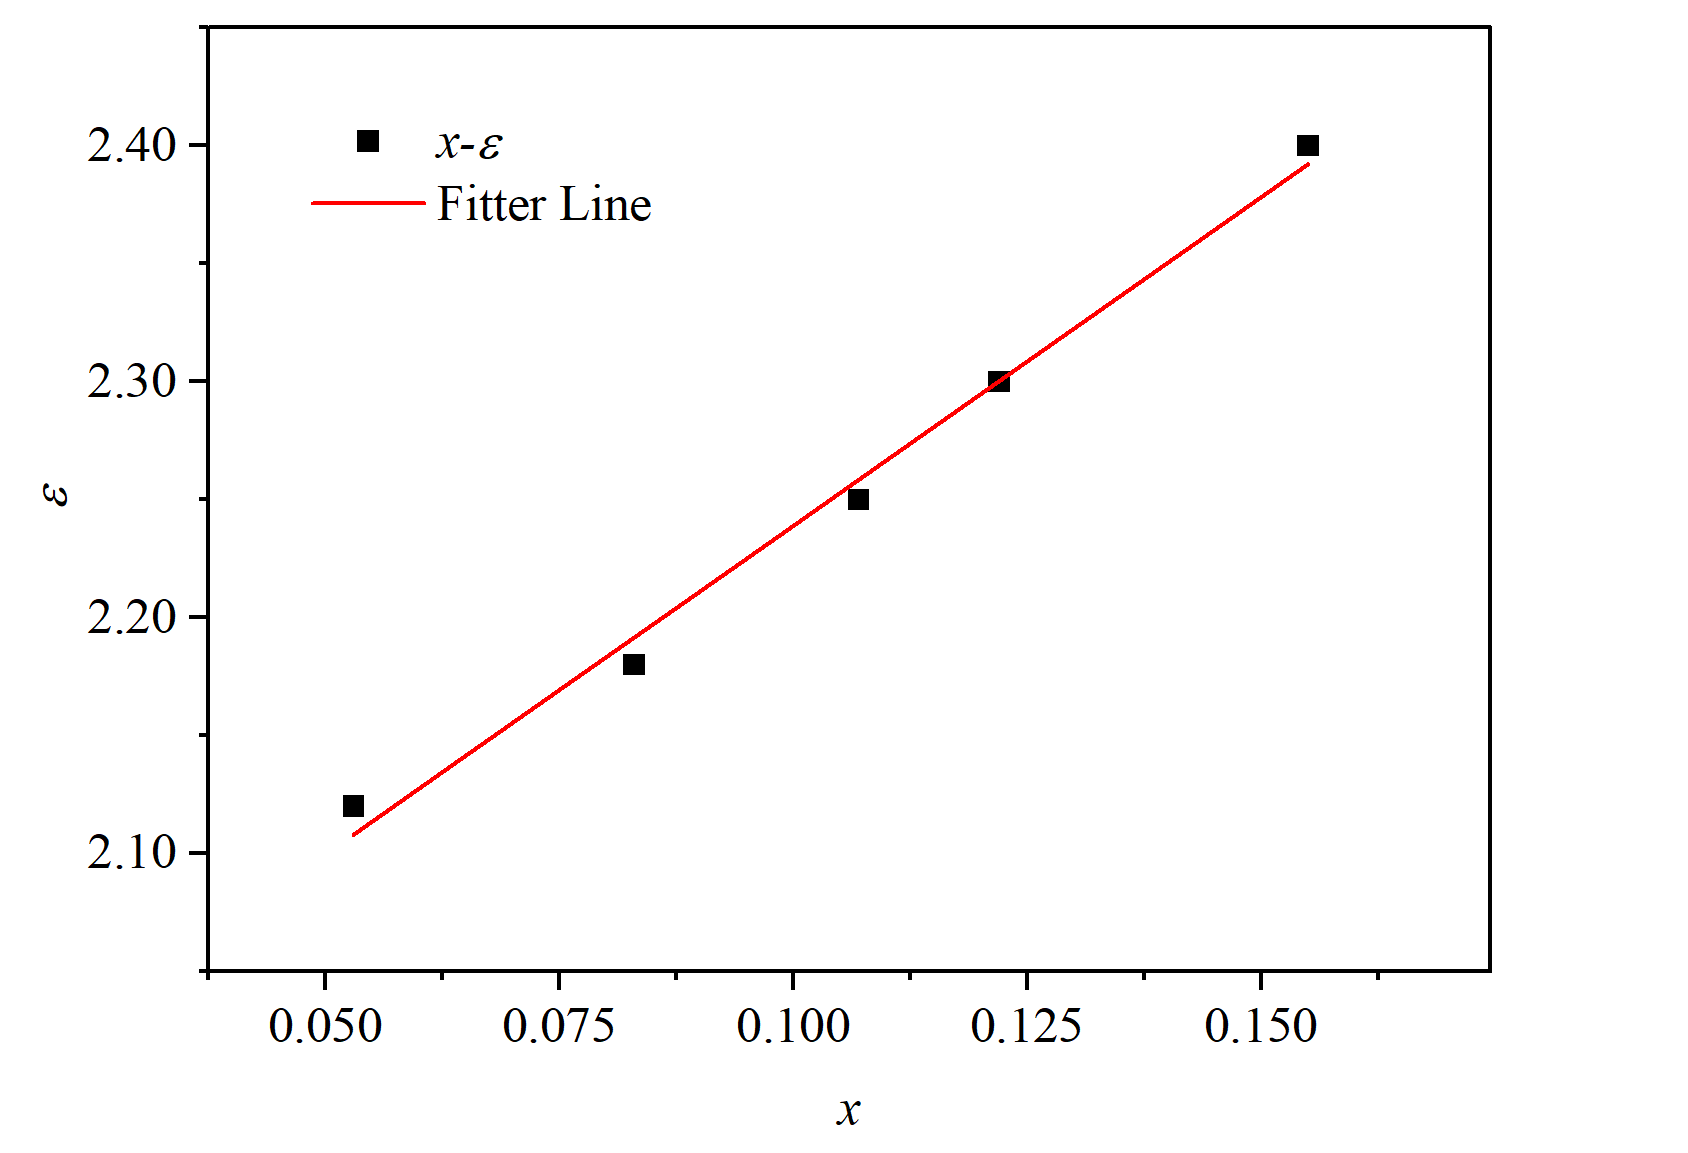
\includegraphics[width=.7\textwidth]{figures/1-1.png}
    \caption{介电常数-摩尔浓度的拟合直线}
    \label{fig:2}
\end{figure}

\subsection{溶液的密度}

本次实验中,测定正丁醇-环己烷溶液在$25.00\mathrm{{}^\circ C}$时的密度,测量结果如表 \ref{tab:3}。

\begin{table}[htbp]
    \centering
    \caption{不同摩尔浓度的正丁醇-环己烷溶液的密度}
    \begin{tabular}{ccccc}
    \toprule
        $x$ & $\rho_1/\mathrm{g\cdot cm^{-3}}$ & $\rho_2/\mathrm{g\cdot cm^{-3}}$ & $\rho_3/\mathrm{g\cdot cm^{-3}}$ & $\bar{\rho}/\mathrm{g\cdot cm^{-3}}$ \\
    \midrule
    0.000 & 0.77835 & 0.77836 & 0.77835 & 0.77835 \\
    0.053 & 0.77418 & 0.77418 & 0.77418 & 0.77418 \\
    0.083 & 0.77463 & 0.77462 & 0.77462 & 0.77462 \\
    0.107 & 0.77510 & 0.77512 & 0.77512 & 0.77511 \\
    0.122 & 0.77534 & 0.77533 & 0.77533 & 0.77533 \\
    0.155 & 0.77596 & 0.77594 & 0.77595 & 0.77595 \\
    1.000 & 0.80571 & 0.80572 & 0.80572 & 0.80572 \\
    \bottomrule
    \end{tabular}
    \label{tab:3}
\end{table}

假设密度仪的允差为$1\times 10^{-5}\mathrm{~g}$,则密度仪的误差为:
\begin{equation*}
    \sigma_{\rho} = \frac{1\times 10^{-5}}{\sqrt{3}} = 5.8 \times 10^{-6}
\end{equation*}
三次测量取平均后,密度误差为:
\begin{equation*}
    \sigma_{\bar{\rho}} = \frac{\sqrt{3}}{3}\sigma_{\rho} = 3.3 \times 10^{-6}
\end{equation*}

对于密度$\rho$-摩尔浓度$x$,进行线性拟合,得到的拟合直线表达式 \eqref{eq:4},图像如图 \ref{fig:3}。
\begin{equation}\label{eq:4}
    \rho/\mathrm{g\cdot cm^{-3}} = (0.01749 \pm 0.00053) x + (0.77322 \pm 0.00006);\quad R^2 = 0.997
\end{equation}

\begin{figure}[htbp]
    \centering
    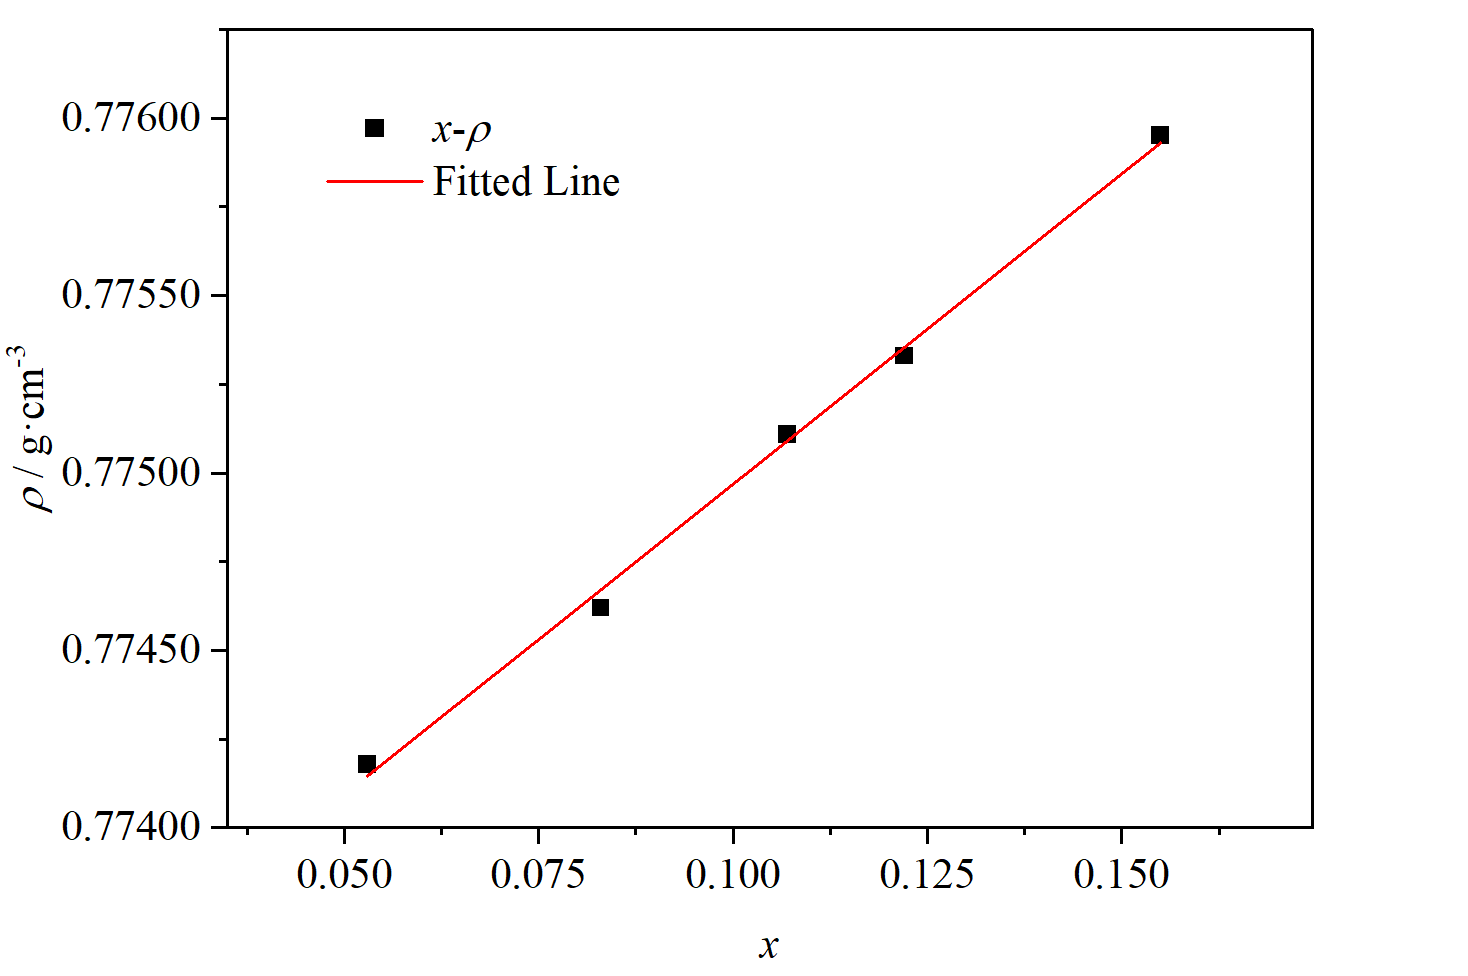
\includegraphics[width=.7\textwidth]{figures/1-2.png}
    \caption{密度-摩尔浓度的拟合直线}
    \label{fig:3}
\end{figure}

\subsubsection{使用比重瓶测定正丁醇的密度}

本次实验中,练习使用了比重瓶,以水为标准溶液,测定正丁醇的密度,数据如表 \ref{tab:5}。

\begin{table}[htbp]
    \centering
    \caption{比重瓶测定密度数据}
    \begin{tabular}{ccccccc}
    \toprule
         液体种类 & $m_0/\mathrm{~g}$ & $m_1/\mathrm{~g}$ & $m_0^\prime/\mathrm{~g}$ & $\Delta m$ & $m_1^\prime/\mathrm{~g}$ & $\Delta m^\prime$\\
    \midrule
        \ce{H_2O} & 19.564 & 23.355 & 4.791 & 19.562 & 23.354 & 4.792\\
        \ce{\textit{n}-BuOH} & 19.548 & 23.401 & 3.853 & 19.549 & 23.399 & 3.856\\
        \bottomrule
    \end{tabular}
    \label{tab:5}
\end{table}

已知$20.9\mathrm{{}^\circ C}$时,水的密度 $\rho_{\ce{H_2O}} = 0.9980\mathrm{~g\cdot cm^{-3}}$,可以求得正丁醇的密度:
\begin{equation*}
    \rho_{\ce{\textit{n}-BuOH}} = \rho_{\ce{H_2O}}\frac{\Delta m_{\ce{\textit{n}-BuOH}}+\Delta m_{\ce{\textit{n}-BuOH}}^\prime}{\Delta m_{\ce{H_2O}}+\Delta m_{\ce{H_2O}}^\prime} = 0.9980\times\frac{3.853+3.856}{4.791+4.792} = 0.8028\mathrm{~g\cdot cm^{-3}}
\end{equation*}

误差计算:
\begin{equation*}
\begin{aligned}
\frac{\partial \rho_{\ce{\textit{n}-BuOH}} }{\partial \Delta m_{\ce{\textit{n}-BuOH}} }&=\frac{\rho_{\ce{H_2O}}}{\Delta m_{\ce{H_2O}} + \Delta m_{\ce{H_2O}}^\prime}=\frac{\left(0.998\right)}{\left(4.791\right) + \left(4.792\right)}=0.1\\
\frac{\partial \rho_{\ce{\textit{n}-BuOH}} }{\partial \Delta m_{\ce{\textit{n}-BuOH}}^\prime }&=\frac{\rho_{\ce{H_2O}}}{\Delta m_{\ce{H_2O}} + \Delta m_{\ce{H_2O}}^\prime}=\frac{\left(0.998\right)}{\left(4.791\right) + \left(4.792\right)}=0.1\\
\frac{\partial \rho_{\ce{\textit{n}-BuOH}} }{\partial \Delta m_{\ce{H_2O}} }&=- \frac{\rho_{\ce{H_2O}} \left(\Delta m_{\ce{\textit{n}-BuOH}} + \Delta m_{\ce{\textit{n}-BuOH}}^\prime\right)}{\left(\Delta m_{\ce{H_2O}} + \Delta m_{\ce{H_2O}}^\prime\right)^{2}}=- \frac{\left(0.998\right) \times \left(\left(3.853\right) + \left(3.856\right)\right)}{\left(\left(4.791\right) + \left(4.792\right)\right)^{2}}=-0.084\\
\frac{\partial \rho_{\ce{\textit{n}-BuOH}} }{\partial \Delta m_{\ce{H_2O}}^\prime }&=- \frac{\rho_{\ce{H_2O}} \left(\Delta m_{\ce{\textit{n}-BuOH}} + \Delta m_{\ce{\textit{n}-BuOH}}^\prime\right)}{\left(\Delta m_{\ce{H_2O}} + \Delta m_{\ce{H_2O}}^\prime\right)^{2}}=- \frac{\left(0.998\right) \times \left(\left(3.853\right) + \left(3.856\right)\right)}{\left(\left(4.791\right) + \left(4.792\right)\right)^{2}}=-0.084\\
\end{aligned}
\end{equation*}
\begin{equation*}
\begin{aligned}
\sigma_{\rho_{\ce{\textit{n}-BuOH}}}&=\left[\left(\frac{\partial \rho_{\ce{\textit{n}-BuOH}} }{\partial \Delta m_{\ce{\textit{n}-BuOH}} } \sigma_{\Delta m_{\ce{\textit{n}-BuOH}}}\right)^2+\left(\frac{\partial \rho_{\ce{\textit{n}-BuOH}} }{\partial \Delta m_{\ce{\textit{n}-BuOH}}^\prime } \sigma_{\Delta m_{\ce{\textit{n}-BuOH}}^\prime}\right)^2+\left(\frac{\partial \rho_{\ce{\textit{n}-BuOH}} }{\partial \Delta m_{\ce{H_2O}} } \sigma_{\Delta m_{\ce{H_2O}}}\right)^2+\right.\\
& \left.\left(\frac{\partial \rho_{\ce{\textit{n}-BuOH}} }{\partial \Delta m_{\ce{H_2O}}^\prime } \sigma_{\Delta m_{\ce{H_2O}}^\prime}\right)^2\right]^{\frac12}\\  
&=\sqrt{\left(0.1 \times 0.0008\right)^2+\left(0.1 \times 0.0008\right)^2+\left(-0.084 \times 0.0008\right)^2+\left(-0.084 \times 0.0008\right)^2}\\
&=\sqrt{\left(8.3 \times 10^{-5}\right)^2+\left(8.3 \times 10^{-5}\right)^2+\left(-6.7 \times 10^{-5}\right)^2+\left(-6.7 \times 10^{-5}\right)^2}\\
&=0.00015\ \mathrm{~m^3\cdot mol^{-1}}
\end{aligned}
\end{equation*}
最终求得正丁醇密度
\begin{equation*}
\rho_{\ce{\textit{n}-BuOH}}=\left (0.8028 \pm 0.00015 \right )\ \mathrm{~m^3\cdot mol^{-1}}
\end{equation*}

这与通过数字密度仪测得的正丁醇密度仍有较小的、超出误差范围的偏差,可能是由于比重瓶自身的仪器误差导致的。

\subsection{正丁醇的摩尔折射率}

使用阿贝折射仪,测定正丁醇的折射率如表 \ref{tab:4} 所示。

\begin{table}[htbp]
    \centering
    \caption{正丁醇的折射率}
    \begin{tabular}{cccc}
    \toprule
         $n_1$ & $n_2$ & $n_3$ & $\bar{n}$ \\
         \midrule
         1.3976 & 1.3974 & 1.3977 & 1.3976\\
         \bottomrule
    \end{tabular}
    \label{tab:4}
\end{table}

假设折射仪的允差为$1\times 10^{-4}$,则密度仪的误差为:
\begin{equation*}
    \sigma_{n} = \frac{1\times 10^{-4}}{\sqrt{3}} = 5.8 \times 10^{-5}
\end{equation*}
三次测量取平均后,密度误差为:
\begin{equation*}
    \sigma_{\bar{n}} = \frac{\sqrt{3}}{3}\sigma_{n} = 3.3 \times 10^{-5}
\end{equation*}

根据表 \ref{tab:4},可以计算正丁醇的摩尔折射率$R$及其误差:
\begin{equation*}
R=\frac{74.12 n^{2} - 74.12}{\rho \left(n^{2} + 2\right)}=\frac{74.12 \times \left(1.3976\right)^{2} - 74.12}{\left(807520\right) \times \left(\left(1.3976\right)^{2} + 2\right)}=2.2133 \times 10^{-5}\mathrm{~ m^3\cdot mol^{-1}}
\end{equation*}
\begin{equation*}
\begin{aligned}
\frac{\partial R }{\partial n }&=\frac{444.72 n}{\rho \left(n^{2} + 2\right)^{2}}=\frac{444.72 \times \left(1.3976\right)}{\left(807520\right) \times \left(\left(1.3976\right)^{2} + 2\right)^{2}}=4.9 \times 10^{-5}\\
\frac{\partial R }{\partial \rho }&=\frac{74.12 \cdot \left(1 - n^{2}\right)}{\rho^{2} \left(n^{2} + 2\right)}=\frac{74.12 \times \left(1 - \left(1.3976\right)^{2}\right)}{\left(807520\right)^{2} \times \left(\left(1.3976\right)^{2} + 2\right)}=-2.7 \times 10^{-11}\\
\end{aligned}
\end{equation*}
\begin{equation*}
\begin{aligned}
\sigma_{R}&=\sqrt{\left(\frac{\partial R }{\partial n } \sigma_{n}\right)^2+\left(\frac{\partial R }{\partial \rho } \sigma_{\rho}\right)^2}\\
&=\sqrt{\left(4.9 \times 10^{-5} \times 0.00033\right)^2+\left(-2.7 \times 10^{-11} \times 3.3\right)^2}\\
&=\sqrt{\left(1.6 \times 10^{-8}\right)^2+\left(-9.0 \times 10^{-11}\right)^2}\\
&=1.6 \times 10^{-8}\mathrm{~ m^3\cdot mol^{-1}}
\end{aligned}
\end{equation*}
最终,正丁醇的摩尔折射率$R$可以表示为:
\begin{equation*}
R=(2.2133  \pm 0.0016 )\times 10^{-5}\mathrm{~ m^3\cdot mol^{-1}}
\end{equation*}

\subsection{正丁醇偶极矩的计算}

由线性拟合结果 \eqref{eq:3}、\eqref{eq:4} 可得以下参数:

\begin{itemize}
    \item Fitted Line of $\varepsilon-x$:
    \begin{itemize}
        \item Intercept:$\varepsilon_1 = 1.9602 \pm 0.0166$
        \item Slope:$a = 2.7861\pm 0.1514$
    \end{itemize}
    \item Fitted Line of $\rho-x$:
    \begin{itemize}
        \item Intercept:$\rho_1 = (0.77322 \pm 0.00006) \times 10^{3} \mathrm{~kg\cdot m^{-3}}$
        \item Slope:$b = (0.01749\pm 0.00053)\times 10^{3}\mathrm{~kg\cdot m^{-3}} $
    \end{itemize}
\end{itemize}



根据Hedestrand经验公式:
\begin{equation}\label{eq:5}
    \bar{P}_2^\infty = A(M_2-bB)+aC
\end{equation}
其中:

\begin{itemize}
    \item $A$及其不确定度的计算:
    \begin{equation*}
A=\frac{\varepsilon - 1}{\rho \left(\varepsilon + 2\right)}=\frac{\left(1.9602\right) - 1}{\left(773.22\right) \times \left(\left(1.9602\right) + 2\right)}=0.0003136\ \mathrm{~m^3\cdot kg^{-1}}
\end{equation*}
\begin{equation*}
\begin{aligned}
\frac{\partial A }{\partial \varepsilon }&=\frac{3}{\rho \left(\varepsilon + 2\right)^{2}}=\frac{3}{\left(773.22\right) \times \left(\left(1.9602\right) + 2\right)^{2}}=0.00025\\        
\frac{\partial A }{\partial \rho }&=\frac{1 - \varepsilon}{\rho^{2} \left(\varepsilon + 2\right)}=\frac{1 - \left(1.9602\right)}{\left(773.22\right)^{2} \times \left(\left(1.9602\right) + 2\right)}=-4.1 \times 10^{-7}\\
\end{aligned}
\end{equation*}
\begin{equation*}
\begin{aligned}
\sigma_{A}&=\sqrt{\left(\frac{\partial A }{\partial \varepsilon } \sigma_{\varepsilon}\right)^2+\left(\frac{\partial A }{\partial \rho } \sigma_{\rho}\right)^2}\\
&=\sqrt{\left(0.00025 \times 0.0017\right)^2+\left(-4.1 \times 10^{-7} \times 0.0033\right)^2}\\
&=\sqrt{\left(4.1 \times 10^{-7}\right)^2+\left(-1.3 \times 10^{-9}\right)^2}\\
&=4.1 \times 10^{-7}\ \mathrm{~m^3\cdot kg^{-1}}
\end{aligned}
\end{equation*}
\begin{equation*}
A= (3.136 \pm 0.0041) \times 10^{-4} \ \mathrm{~m^3\cdot kg^{-1}}
\end{equation*}

\item $B$及其不确定度的计算:
\begin{equation*}
B=\frac{0.08416}{\rho}=\frac{0.08416}{\left(773.22\right)}=0.0001088\ \mathrm{~m^3\cdot mol^{-1}}
\end{equation*}
\begin{equation*}
\begin{aligned}
\frac{\partial B }{\partial \rho }&=- \frac{0.08416}{\rho^{2}}=- \frac{0.08416}{\left(773.22\right)^{2}}=-1.4 \times 10^{-7}\\
\end{aligned}
\end{equation*}
\begin{equation*}
\begin{aligned}
\sigma_{B}&=\sqrt{\left(\frac{\partial B }{\partial \rho } \sigma_{\rho}\right)^2}\\
&=\sqrt{\left(-1.4 \times 10^{-7} \times 0.0033\right)^2}\\   
&=\sqrt{\left(-4.6 \times 10^{-10}\right)^2}\\
&=4.6 \times 10^{-10}\ \mathrm{~m^3\cdot mol^{-1}}
\end{aligned}
\end{equation*}
\begin{equation*}
B=(1.088 \pm 0.0000046)\times 10^{-4} \ \mathrm{~m^3\cdot mol^{-1}}
\end{equation*}

\item $C$及其不确定度的计算:
\begin{equation*}
C=\frac{0.25248}{\rho \left(\varepsilon + 2\right)^{2}}=\frac{0.25248}{\left(773.22\right) \times \left(\left(1.9602\right) + 2\right)^{2}}=2.082 \times 10^{-5}\ \mathrm{~m^3\cdot mol^{-1}}
\end{equation*}
\begin{equation*}
\begin{aligned}
\frac{\partial C }{\partial \varepsilon }&=- \frac{0.50496}{\rho \left(\varepsilon + 2\right)^{3}}=- \frac{0.50496}{\left(773.22\right) \times \left(\left(1.9602\right) + 2\right)^{3}}=-1.1 \times 10^{-5}\\
\frac{\partial C }{\partial \rho }&=- \frac{0.25248}{\rho^{2} \left(\varepsilon + 2\right)^{2}}=- \frac{0.25248}{\left(773.22\right)^{2} \times \left(\left(1.9602\right) + 2\right)^{2}}=-2.7 \times 10^{-8}\\
\end{aligned}
\end{equation*}
\begin{equation*}
\begin{aligned}
\sigma_{C}&=\sqrt{\left(\frac{\partial C }{\partial \varepsilon } \sigma_{\varepsilon}\right)^2+\left(\frac{\partial C }{\partial \rho } \sigma_{\rho}\right)^2}\\
&=\sqrt{\left(-1.1 \times 10^{-5} \times 0.0017\right)^2+\left(-2.7 \times 10^{-8} \times 0.0033\right)^2}\\
&=\sqrt{\left(-1.7 \times 10^{-8}\right)^2+\left(-8.9 \times 10^{-11}\right)^2}\\
&=1.7 \times 10^{-8}\ \mathrm{~m^3\cdot mol^{-1}}
\end{aligned}
\end{equation*}
\begin{equation*}
C=(2.082  \pm 0.0017) \times 10^{-5}\ \mathrm{~m^3\cdot mol^{-1}}
\end{equation*}
\end{itemize}


将$A,B,C$带入Hedestrand经验公式 \eqref{eq:5} 中,得到$\bar{P}_2^\infty$及其不确定度:
\begin{align*}
\bar{P}_2^\infty &=A \left(- B b + 0.07412\right) + C a \\
&=\left(0.0003136\right) \times \left(- \left(0.0001088\right) \times \left(17.49\right) + 0.07412\right) + \left(2.082 \times 10^{-5}\right) \times \left(2.7861\right)\\
&=8.065 \times 10^{-5}\ \mathrm{~m^3\cdot mol^{-1}}
\end{align*}
\begin{equation*}
\begin{aligned}
\frac{\partial \bar{P}_2^\infty }{\partial A }&=- B b + 0.07412=- \left(0.0001088\right) \times \left(17.49\right) + 0.07412=0.072\\    
\frac{\partial \bar{P}_2^\infty }{\partial b }&=- A B=- \left(0.0003136\right) \times \left(0.0001088\right)=-3.4 \times 10^{-8}\\
\frac{\partial \bar{P}_2^\infty }{\partial B }&=- A b=- \left(0.0003136\right) \times \left(17.49\right)=-0.0055\\
\frac{\partial \bar{P}_2^\infty }{\partial a }&=C=\left(2.082 \times 10^{-5}\right)=2.1 \times 10^{-5}\\
\frac{\partial \bar{P}_2^\infty }{\partial C }&=a=\left(2.7861\right)=2.8\\
\end{aligned}
\end{equation*}
\begin{equation*}
\begin{aligned}
\sigma_{\bar{P}_2^\infty}&=\sqrt{\left(\frac{\partial \bar{P}_2^\infty }{\partial A } \sigma_{A}\right)^2+\left(\frac{\partial \bar{P}_2^\infty }{\partial b } \sigma_{b}\right)^2+\left(\frac{\partial \bar{P}_2^\infty }{\partial B } \sigma_{B}\right)^2+\left(\frac{\partial \bar{P}_2^\infty }{\partial a } \sigma_{a}\right)^2+\left(\frac{\partial \bar{P}_2^\infty }{\partial C } \sigma_{C}\right)^2}\\
&=\left[\left(0.072 \times 4.1 \times 10^{-7}\right)^2+\left(-3.4 \times 10^{-8} \times 0.53\right)^2+\left(-0.0055 \times 4.6 \times 10^{-10}\right)^2+\right.\\
&\left.\left(2.1 \times 10^{-5} \times 0.15\right)^2+\left(2.8 \times 1.7 \times 10^{-8}\right)^2\right]^{\frac12}\\   
&=\sqrt{\left(3.0 \times 10^{-8}\right)^2+\left(-1.8 \times 10^{-8}\right)^2+\left(-2.5 \times 10^{-12}\right)^2+\left(3.2 \times 10^{-6}\right)^2+\left(4.7 \times 10^{-8}\right)^2}\\   
&=3.2 \times 10^{-6}\ \mathrm{~m^3\cdot mol^{-1}}
\end{aligned}
\end{equation*}
\begin{equation*}
\bar{P}_2^\infty= (8.065  \pm 0.315) \times 10^{-5} \ \mathrm{~m^3\cdot mol^{-1}}
\end{equation*}

最终,计算得到正丁醇的偶极矩及其不确定度:
\begin{equation}\label{eq:7}
    \begin{aligned}
    \mu_{\ce{\textit{n}-BuOH}} &= 12.81\sqrt{\left(\frac{\bar{P}_2^\infty}{\mathrm{m^3\cdot mol^{-1}}}-\frac{R}{\mathrm{m^3\cdot mol^{-1}}}\right)\left(\frac{T}{\mathrm{K}}\right)} \mathrm{~D} \\
    &= 12.81\sqrt{(8.065-2.2133) \times 10^{-5}\times(273.15+20.9)} \mathrm{~D}\\
    &= 1.680 \mathrm{~D}
\end{aligned}
\end{equation}
\begin{equation*}
\begin{aligned}
\frac{\partial \mu_{\ce{\textit{n}-BuOH}} }{\partial \bar{P}_2^\infty }&=\frac{6.405 \sqrt{T \left(\bar{P}_2^\infty - R\right)}}{\bar{P}_2^\infty - R}=\frac{6.405 \times \sqrt{\left(294.05\right) \times \left(\left(8.065 \times 10^{-5}\right) - \left(2.2133 \times 10^{-5}\right)\right)}}{\left(8.065 \times 10^{-5}\right) - \left(2.2133 \times 10^{-5}\right)}=1.4 \times 10^{4}\\
\frac{\partial \mu_{\ce{\textit{n}-BuOH}} }{\partial R }&=- \frac{6.405 \sqrt{T \left(\bar{P}_2^\infty - R\right)}}{\bar{P}_2^\infty - R}\\
&=- \frac{6.405 \times \sqrt{\left(294.05\right) \times \left(\left(8.065 \times 10^{-5}\right) - \left(2.2133 \times 10^{-5}\right)\right)}}{\left(8.065 \times 10^{-5}\right) - \left(2.2133 \times 10^{-5}\right)}=-1.4 \times 10^{4}\\
\frac{\partial \mu_{\ce{\textit{n}-BuOH}} }{\partial T }&=\frac{6.405 \sqrt{T \left(\bar{P}_2^\infty - R\right)}}{T}=\frac{6.405 \times \sqrt{\left(294.05\right) \times \left(\left(8.065 \times 10^{-5}\right) - \left(2.2133 \times 10^{-5}\right)\right)}}{\left(294.05\right)}=0.0029\\
\end{aligned}
\end{equation*}
\begin{equation*}
\begin{aligned}
\sigma_{\mu_{\ce{\textit{n}-BuOH}}}&=\sqrt{\left(\frac{\partial \mu_{\ce{\textit{n}-BuOH}} }{\partial \bar{P}_2^\infty } \sigma_{\bar{P}_2^\infty}\right)^2+\left(\frac{\partial \mu_{\ce{\textit{n}-BuOH}} }{\partial R } \sigma_{R}\right)^2+\left(\frac{\partial \mu_{\ce{\textit{n}-BuOH}} }{\partial T } \sigma_{T}\right)^2}\\
&=\sqrt{\left(1.4 \times 10^{4} \times 3.2 \times 10^{-6}\right)^2+\left(-1.4 \times 10^{4} \times 1.6 \times 10^{-8}\right)^2+\left(0.0029 \times 0.058\right)^2}\\
&=\sqrt{\left(0.045\right)^2+\left(-0.00023\right)^2+\left(0.00017\right)^2}\\
&=0.045\mathrm{~D}
\end{aligned}
\end{equation*}
最终,得到正丁醇的偶极矩:
\begin{equation*}
\mu_{\ce{\textit{n}-BuOH}}=\left (1.68 \pm 0.045 \right )\mathrm{~D} 
\end{equation*}

\section{结果与讨论}

% 对自己实验结果可靠性和可信度的论证和评价(如:误差的分析和估算、结果有效数字位数的确定等, 误差分析不要求面面俱到)
\subsection{误差分析}

本次实验的误差分析已在数据处理过程中计算。

\subsection{思考题}

\subsubsection{思考题1}

\begin{enumerate}
    \item \textbf{分子在电场中的极化有哪些类型?}
    \begin{itemize}
        \item \textbf{原子极化}::当一个原子或分子处于外部电场中时,其电子云会受到电场的影响而相对于原子核产生位移。这导致电子云的中心与原子核的中心不再重合,从而形成一个瞬时偶极矩。这种因电子云变形而产生的极化被称为原子极化或电子极化。
        \item \textbf{电子极化}:是指当外部电场作用于一个原子或分子时,其电子云受到电场的影响而发生位移。这种位移导致电子云的中心与原子核的中心不再重合,形成了瞬时的偶极矩。
        \item \textbf{转向极化(取向极化)}:某些分子,如水分子,本身就具有永久的偶极矩。当它们处于外部电场中时,这些偶极分子会尝试与电场方向对齐。在一个随机取向的偶极分子集合中施加电场会使得这些分子倾向于按照电场方向排列,从而增加整体的偶极矩。这种现象称为转向极化或取向极化。
    \end{itemize}
    \item \textbf{本次实验如何考虑这些极化类型的贡献?}
    \begin{itemize}
        \item 本次实验中,考虑:
        \begin{equation*}
            P_{\text{诱}} = P_E + P_A
        \end{equation*}
        其中,原子极化度$P_A\approx(5.0\%\sim15.0\%)P_{\text{诱}}$。
        \item 本次实验中,测得的:
        \begin{equation*}
            \frac{P_{\text{诱}}}{P} = \frac{\bar{P}_2^\infty - R}{\bar{P}_2^\infty} \times 100\%= \frac{8.065-2.213}{8.065} \times 100\% = 72.6\%
        \end{equation*}
        \item 所以,原子极化度在总极化度中的比例:
        \begin{equation}\label{eq:6}
            P_A = 72.6\%(5.0\%\sim15.0\%)P = (3.6\%\sim11.0\%)P
        \end{equation}
        \item 综上所述,原子极化度比总极化度小一个数量级,因此一定程度上可以忽略。故本次实验中,只考虑电子极化度与转向极化度。
    \end{itemize}
    \item \textbf{忽略原子极化度会引入多大的误差?}
    \begin{itemize}
        \item 根据式 \eqref{tab:4},忽略原子极化度,会导致测得的总极化度比真实的总极化度小$3.6\%\sim11.0\%$。也就是说,测得的总极化度是真实总极化度的$89.0\%\sim 96.4\%$。
        \item 对最终偶极矩结果而言,考虑 \eqref{eq:7},$\bar{P}_2^\infty - R$是真实值的
        \begin{equation*}
            \frac{(89.0\%\sim 96.4\%)-(1-72.56\%)}{72.56\%} = (85.0\%\sim 95.0\%)
        \end{equation*}
        \item 考虑偶极矩,测得偶极矩是真实偶极矩的
        \begin{equation*}
            \sqrt{(85.0\%\sim 95.0\%)} = (92.2\%\sim 97.5\%)
        \end{equation*}
        \item 所以,对于正丁醇偶极矩而言,忽略原子极化度会引起的误差
        \begin{equation*}
            \sigma_{P_A} = -(3.5\%\sim7.8\%)
        \end{equation*}
    \end{itemize}
\end{enumerate}

\subsubsection{思考题2}

\begin{itemize}
    \item \textbf{考虑电容器的误差对结果的影响}
    \begin{itemize}
        \item 本次实验的数据处理中,在 \ref{cap:1} 中溶液的介电常数的计算一部分,已经考虑了当电容计有着 $\pm 0.01\mathrm{~pF}$ 的最大读数误差(即允差)所带来的误差。
        \item 在 \ref{cap:1} 中,根据表 \ref{tab:2} 与拟合直线的表达式 \eqref{eq:3} 可知:
        \begin{itemize}
            \item 由于电容的测定值进过两次平均,对于介电常数的相对误差较小($\sim 0.2\%$);
            \item 但是,拟合直线表达式 \eqref{eq:3} 中,斜率的相对误差为$6\%$,截距的相对误差为$1\%$;
        \end{itemize}
        由此可知,对最终结果而言,电容计的误差并不是构成最终误差的主要因素,最终误差主要是由最小二乘法计算回归直线时,由于数据点的噪声,在拟合过程中引入的误差。
        \item 因此,电容器的误差最终结果的影响可以忽略不计。
    \end{itemize}
\end{itemize}

\subsubsection{思考题3}

\begin{itemize}
    \item \textbf{室温变化对最终结果的影响}

    考虑室温增加$5^\circ C$时的情况:
    \begin{itemize}
        \item 根据公式 \eqref{eq:8},环己烷的介电常数$\varepsilon_{\ce{CyH}}$:
        \begin{align*}
            \varepsilon_{\ce{CyH}}^\prime &= 2.023 - 0.0016\left(\frac{T}{\mathrm{K}}-293\right)\\
            &= 2.203 - 0.0016\left((273.15+25.9)-293\right)\\
            &= 2.022
        \end{align*}
        \item 根据公式 \eqref{eq:9},电容器的分布电容$C_{\text{d}}$:
        \begin{equation*}
            C_{\text{d}}^\prime = C_{\text{air}}^\prime - \frac{C_{\ce{CyH}}^\prime-C_{\text{air}}^\prime}{\varepsilon_{\ce{CyH}}^\prime-1} = 4.25 -\frac{7.02-4.25}{2.022-1} = 1.540\mathrm{~pF} 
        \end{equation*}
        有
        \begin{equation*}
            \Delta C_{\text{d}} = C_{\text{d}}^\prime - C_{\text{d}} = 1.540 - 1.537 = 0.003\mathrm{~pF} 
        \end{equation*}
        \item 根据式 \eqref{eq:10},电容器分布电容的误差$\sigma_{C_{\text{d}}}$:
        \begin{equation*}
            \sigma_{C_{\text{d}}} = 0.006 > 0.003 = \Delta C_{\text{d}}
        \end{equation*}
    \end{itemize}

    \item 综上所述,即使温度变化$5^\circ C$,其所造成的误差仍然小于其他因素的误差。更何况,温度的实际误差不可能超过$5^\circ C$。
    \item 因此,温度的变化对本实验造成的影响可以忽略不计。
\end{itemize}

\subsection{总结}

本实验通过稀溶液法测定正丁的偶极矩。首先,利用数字密度仪和精密电容测量仪来测定正丁醇-环己烷溶液的密度与电容,通过拟合电容、密度与摩尔浓度的直线,结合Hedestrand经验公式,求得正丁醇的总摩尔极化度$\bar{P}_2^\infty = (8.065\pm 0.315) \times 10^{-5}\mathrm{~m^3\cdot mol^{-1}}$;其次,使用阿贝折射仪测定正丁醇的折射率,进而求得其摩尔折射率也就是电子极化度$R=P_E=(2.2133  \pm 0.0016 )\times 10^{-5}\mathrm{~ m^3\cdot mol^{-1}}$;最终,通过转向极化度计算得到正丁醇的偶极矩$\mu_{\ce{\textit{n}-BuOH}}=\left (1.68 \pm 0.045 \right )\mathrm{~D} $。

查阅文献\cite{haynes2016crc}可知,正丁醇的偶极矩$\mu_{\ce{\textit{n}-BuOH},0}=\left (1.66 \pm 0.03 \right )\mathrm{~D} $。由此可见,本次实验测得的正丁醇偶极矩在文献值的误差范围内,可以认为两者没有显著性区别。


\subsection{意见与建议}

\begin{itemize}
    \item \textbf{仪器误差的改进}:本次实验中,所使用的阿贝折射仪与数字密度仪均达到了万分之一的精确度,但是分析天平的精确度为千分之一,电容器的精确度更是只有百分之一,这大大限制了实验结果的精确性。为了提高实验的精确度,可以使用万分之一的分析天平与万分之一精确度的电容器,这样可以使得结果的精确性大幅增加。
    \item \textbf{溶液配置的改进}:本次实验中,虽然并没有必要配置恰好为指定浓度的溶液,但溶液配置的过程比较繁琐,给同学们增加了许多不必要的麻烦,大大限制了实验的速度。为此,可以使用移液枪辅助进行溶液的配置,而不是使用移液管。这样可以增加同学们的实验效率。
    \item \textbf{有机物挥发的问题}:本次实验中,测定电容前需要将电容器使用吹风机吹干。然而电容器中,残留有较多的正丁醇与环己烷,这些有机物会完全会发到实验室的空气中。虽然正丁醇、环己烷的毒性较弱,但长期暴露在正丁醇、环己烷的蒸气中,会对眼睛、喉咙具有一定的刺激性,吸入蒸气也会有一定的慢性毒性。因此,建议如果条件允许的话,在实验台上配备建议的通风装置或在通风橱内进行吹干,如果这些均无法满足,则需要尽可能保证实验室通风,实验时要开门开窗,尽可能减少空气中有机物的浓度。
\end{itemize}

\bibliography{reference}

\end{document}